\documentclass[a4paper,12pt]{jsreport}
\usepackage{bm}
\usepackage[dvipdfmx]{graphicx}
\usepackage{ascmac}
\usepackage[hang,small,bf]{caption}
\usepackage[subrefformat=parens]{subcaption}
\captionsetup{compatibility=false}
\usepackage{geometry}
% ページの余白を1.25インチにする
\geometry{
    left=1.25truein,
    right=1.25truein,
    top=1.25truein,
    bottom=1.25truein,
}
\usepackage{etoolbox}
\patchcmd{\chapter}{\cleardoublepage}{}{}{}
\patchcmd{\chapter}{\clearpage}{}{}{}

\title{ミリ波を用いた地中埋設物の位置と形状の推定}
\author{廣瀬夏秋研究室\\
学籍番号03-210499 高原陽太}


\begin{document}
\maketitle
\tableofcontents
\clearpage
\chapter{はじめに→必須訂正}
\section{研究背景}
 電波を利用して地中を非破壊的に探知する地中レーダー探査技術(GPR)は地中埋設物探査や遺跡調査、地下水流
調査など多くの応用分野を持つ\cite{radar1}\cite{radar2}。GPRは特定周波数範囲の電磁波を用いて行われる。
電磁波は地中を伝搬し、土壌中にて誘電率が異なる物質の境界面で反射を起こす。そのため埋設物の材料物質と
土壌の誘電率の違いを利用して埋設物の検知を行う。
\\ この埋設物探査に焦点を当てたい。工事のための地中調査を行う際、地中の埋設物の有無及びそれがどういったものであるか
を特定することは必須である。特にガス管や水道管などが道路工事現場に埋まっているものの代表例として
挙げられる。そこで実際に工事を施工する前の調査段階でそれら埋設物の詳しい情報を得ておくことが重要となる。
\\ しかし実際のレーダー波形は電磁波の散乱、屈折などの波動現象によって元の埋設物の形状とは異なり、解釈
することが難しい。勿論元の形状に戻すための処理は存在し、マイグレーションと呼ばれる。


\begin{figure}[h]
  \begin{center}
   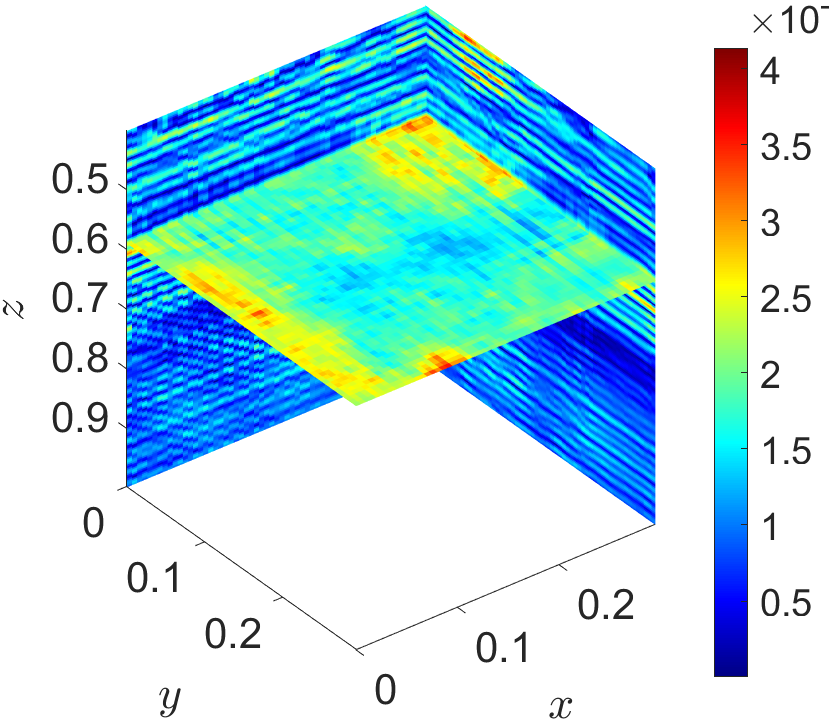
\includegraphics[width=7cm]{./image/0918.png}
   
  \caption{鉄パイプをGPRによって可視化したもの}\label{鉄パイプをGPRによって可視化したもの}
  \end{center}
  \end{figure}

 また、GPRの基本的な構造として一対の送受信アンテナを地面に照射するものがある。しかしこの方法で計測を行う場合、
多数の計測を行うため膨大な時間が必要である。ゆえに計測の労力を減らすことが検討されてきた。そのため、計測点を減らす
ために、圧縮センシングと呼ばれる、スパース性を持った信号を計測する際に、少ない計測点から本来の信号を復元する手法が
ある。この手法によってより少ない処理時間で埋設物を推定することができる。

\section{研究の目的}
 本研究の目的はガス管や水道管などの線状物体をモデル化し、地中に埋設されているパイプ管の有無、形状をより少ない計測点
で推定することである。文献\cite{imai}のようにパイプ管のモデルを考えることでスパース性を持つ箇所の計算を省き、より高速化を図る。
また、線状物体は照射される偏波の向きによって得られる情報が異なる。ゆえに偏波の情報もデータ処理の際に考慮することで
より正確に埋設物の状態を推定することが可能であると思われ、本研究の目的として取り組んでいる。





\chapter{原理と提案手法}
\section{地中レーダーの原理}
 地中レーダーは電磁波の地下物体からの
反射を利用した地下計測手法である。電磁波パルスを地表に置かれた送信アンテナ
から地中に放射し、受信アンテナで受信する。地中を伝搬する電磁波は、土壌中に
誘電率が異なる物質が存在すると反射を起こす性質を持ち、そのため埋設物の材料物質
と誘電率の違いを利用して埋設物の存在を検知することが可能となっている。この反射の様子から
埋設物が埋まっている深度を計測する。
\\ 地中では電磁波速度は導電率、誘電率、透磁率によって決まる。しかしGPRでは10MHzより高い
周波数領域で計測が行われるため、地下媒質の電気的性質は比誘電率$\varepsilon$にのみ左右される。
この時の地中伝搬速度$v$は

\begin{equation}
  v =
  \frac{c}{\sqrt{\varepsilon}} 
  \end{equation}

と書ける。


そして地中の伝搬速度が分かりさえすれば、送信電波が反射波として戻ってくる時間
$\tau$を計測することで図\ref{地中レーダーの様子}のように反射体の深度$d$は次式で導出できる。
\begin{equation}
  d=
  \frac{v \tau}{2} 
  \end{equation}
  
また同様に反射波の振幅も誘電率によって推定できる。図\ref{地中レーダーの様子}のように
誘電率の異なる二層媒質構造の場合について考える。この時上層から入射する電波は境界面で反射を受け
、振幅比$\Gamma$の反射波が発生する。

\begin{figure}[h]
  \begin{center}
   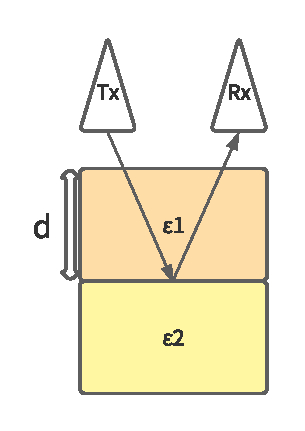
\includegraphics[width=7cm]{./image/radar.pdf}
   
  \caption{地中レーダーの様子}\label{地中レーダーの様子}
  \end{center}
  \end{figure}

反射係数$\Gamma$は境界面で以下のように与えられる。
\begin{equation}
  \Gamma=
  \frac{\sqrt{\varepsilon_{1}}-\sqrt{\varepsilon_{2}}}{\sqrt{\varepsilon_{1}}+\sqrt{\varepsilon_{2}}} 
\label{gamma}  
\end{equation}


式(\ref{gamma})は反射係数が二つの媒質の誘電率のみによって決まることを示している。
\\ これらの情報を測定することで埋設物の位置と材質を推定するのである。

\section{偏波}
 偏波とは図\ref{偏波のイメージ}のように電界と磁界が直行しながら伝搬する波である。偏波を用い、目標物に
照射することで目標物に関する情報を多々得ることができるため、GPRにも用いられている。単に埋設物の反射電力だけで
なく位相も反射によって変わるため、その情報も利用することができるという利点を持つ。
\\ 特に埋設物がパイプなどの線状物体である時に偏波の状態を観測することは重要になる。というのも図\ref{偏波方向とパイプの向きによる反射強度の違い}
のように電磁波の偏波方向と線状物体の方向が一致するとき、大きな反射が起こるのに対して、偏波方向が線状物体と直行すると反射が非常に小さくなってしま
うからである。ゆえにパイプを検出する際には偏波の向きと計測対象の向きを一致させることが必要となる。
\begin{figure}[h]
  \begin{center}
   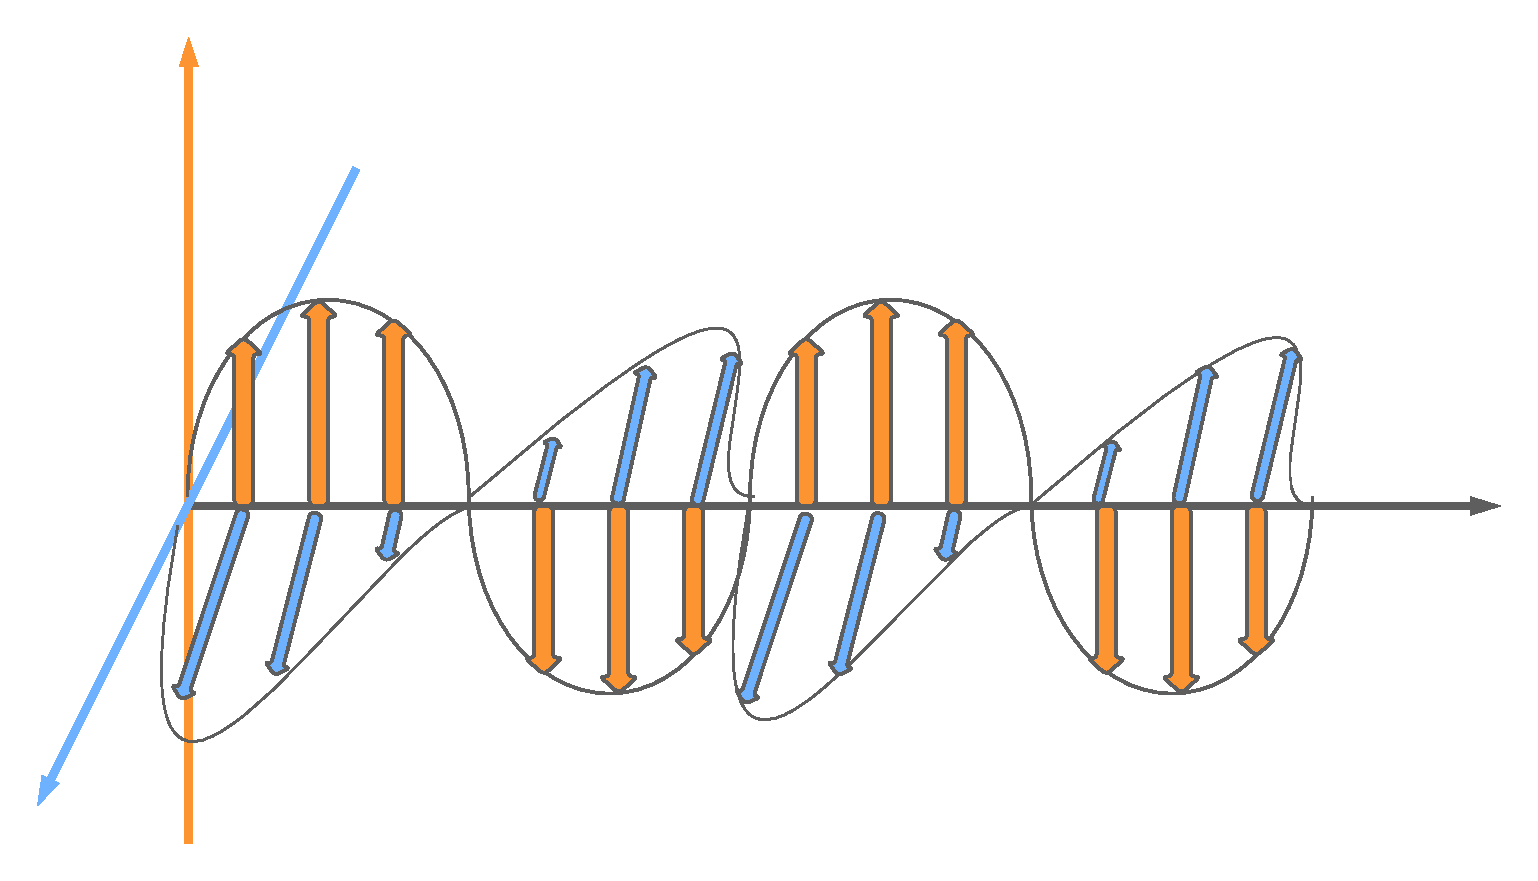
\includegraphics[width=7cm]{./image/wave_propagation.pdf}
  \caption{偏波のイメージ}\label{偏波のイメージ}
  \end{center}
  \end{figure}

  \begin{figure}[h]
    \begin{center}
     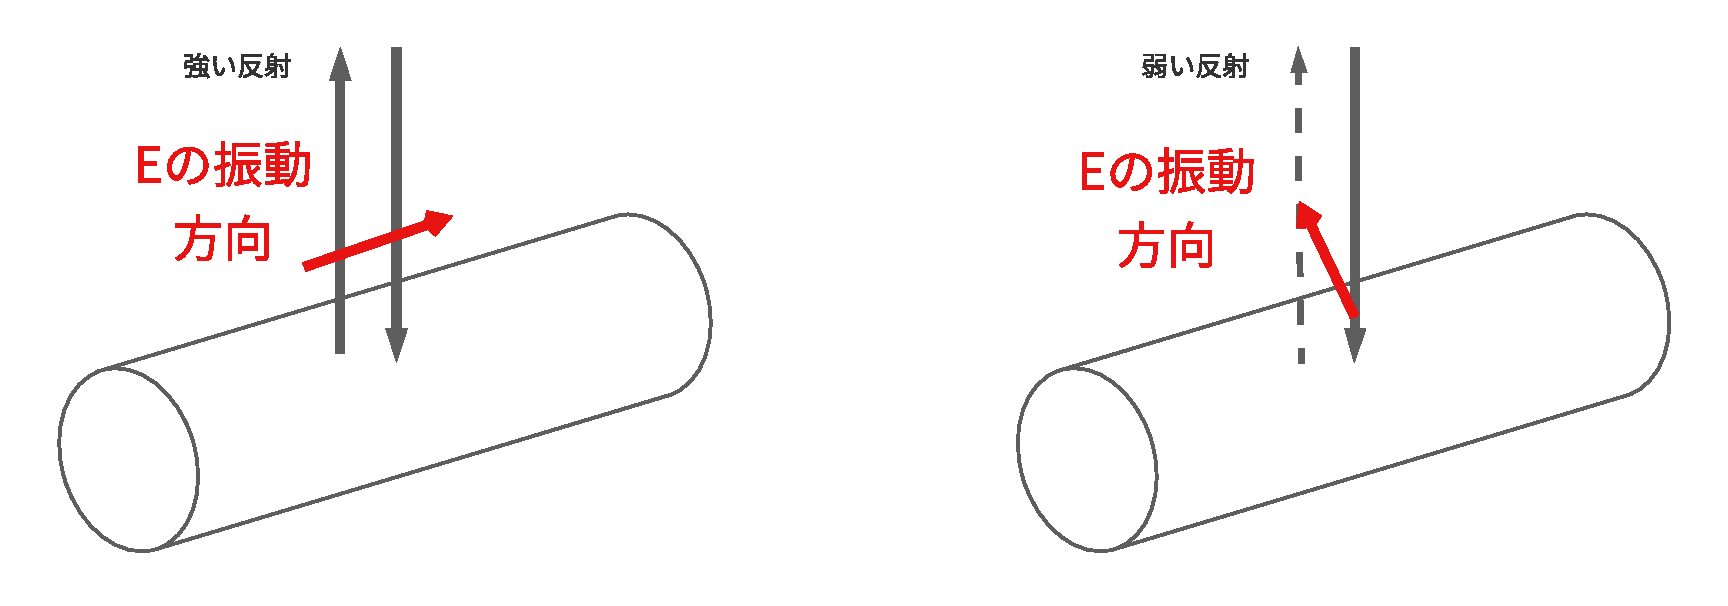
\includegraphics[width=7cm]{./image/polarization.pdf}
    \caption{偏波方向とパイプの向きによる反射強度の違い}\label{偏波方向とパイプの向きによる反射強度の違い}
    \end{center}
    \end{figure}

 \section{圧縮センシング→訂正}
 圧縮センシングとは、対象となる信号をできるだけ少ない観察点数から復元する技術のことである。圧縮技術の多くは、一旦観察信号を
大容量データとして取得した後に圧縮削減するが、圧縮センシングとは観察と圧縮を同時に行うことができ、効率的にデータを取得することが可能である。
\\ 圧縮センシングにおいては「スパース(疎)性」を満たすことが必要である。スパース性とは、ゼロ成分が多く含まれる性質を示し、圧縮センシングでは
ゼロ成分のデータを削減してもキーとなる非ゼロ成分から信号の復元が可能となる。例えば測定データを画像化したものについて考える。理想的な画像では
材質あるいは成分が同じ場合信号強度は等しく、境界面でのみ信号強度が変化すると考えられる。ゆえに境界についての情報が重要となり、画像を境界と
それ以外の情報に分離するような画像変換を行えば、スパース性が高くなり、少ない情報から理想的な画像を再現することができる。


\chapter{従来の手法と提案手法}
\section{従来の手法→訂正}
地中埋設物、主に地雷の検知のためにGPRが用いられている。しかし計測点が多数になり計測時間が膨大になってしまいがちなため
圧縮センシングの手法が利用されてきた。これによって少ない計測点から地中に埋まっている物体の可視化が可能になる。
\\ これらの手法のほとんどが散乱の強度を用いたものであった。しかし強度のみの情報では目的の埋設物とその他関係がない埋設物との区別が困難になってしまう。
\\ 強度以外の情報を用いた手法として\cite{hirose1}~\cite{hirose3}にあるようにテクスチャなどの高次元な計測情報を特徴量として用いたものが挙げられる。
この手法では各計量点において空間、周波数領域における相関を含む特徴量ベクトルを構成する。それらのベクトルは自己組織化マップによって分類される。
\\ また\cite{imai}では地中に埋まっている地雷を模した円柱型のプラスチック模型を探知する際に円形のモデルを仮定して圧縮センシングを行っている。この円形モデル内の
特徴量の一様性を考える。すなわち同じ材質のものは信号強度が一様とする。この一様度合は空間的に疎な分布となる。
\\ 次に実際の計測領域内を測定するがスパース性を考えるとまばらな計測で済む。このまばらなデータを補間する。このデータに対して、上記の一様性を持った円形のモデルと
照らし合わせ、最も類似しているところに地雷が埋まっていると検知する。これによって少ない測定点数、短い計測時間の実現を可能にしている。

\section{提案手法}
 パイプ管をモデル化する際にまず\cite{imai}のように一様とみなせる領域を考える。パイプのような線状の物体は線方向に一様である。
ゆえに線状方向に関しては計測点数を減らすことが可能となる。
\\ それゆえパイプの向きを推定することが必要となる。しかし実際にGPRを用いた時、図\ref{電波の散乱の様子}のようにパイプにぶつかった電磁波はあらゆる方向に散乱し、また
図\ref{偏波方向とパイプの向きによる反射強度の違い}のように電界の向きによって反射波の振幅が大きく異なる。
\\ そのため例えばパイプの向きに垂直に電磁波を照射してしまった場合、反射の大きさによって埋設物を検知するGPR上ではパイプの存在を検知できない。
よって向きがわかってないパイプをGPRによって計測する場合、偏波の向きを水平、垂直に切り替える必要がある。

\begin{figure}[h]
  \begin{center}
   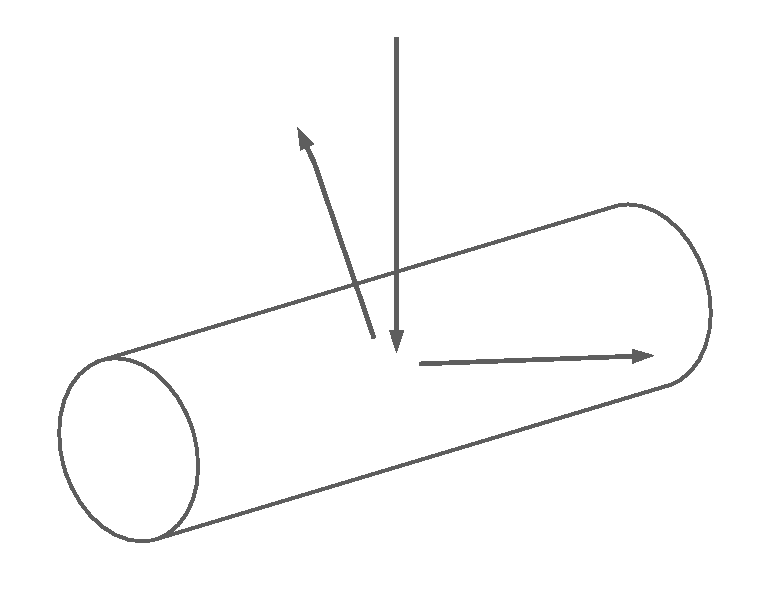
\includegraphics[width=7cm]{./image/scattering.pdf}
  \caption{電波の散乱の様子}\label{電波の散乱の様子}
  \end{center}
  \end{figure}

 逆に言えば、偏波を水平、垂直に照射し、反射波の強さを比較することでパイプの向きがより水平方向あるいは垂直方向
か分かる。ゆえにデータ処理の際、ある測定点での水平偏波、垂直偏波による反射波の強さからパイプの向きが推定でき、
その方向への測定点数を減らすことに繋がる。よって圧縮センシングを行う際、偏波の情報を加味することでより
測定時間の短縮が期待できると考える。

\chapter{実験}
\section{実験概要}
 実際にパイプ管(図\ref{埋設したパイプ})を埋設し、地中レーダーを照射し、測定を行った。図\ref{実験の様子}は使用した
地中レーダーの写真である。図\ref{実験の様子}のアンテナについては図\ref{測定用のアンテナ}を5cm間隔で向かい合わせにし、片方を送信用もう
一方を受信用とすることでデータを測定している。実際のアンテナの測定方向として図\ref{アンテナの動作方向}ようにx軸、y軸ともに
5mm間隔ごとに移動し、それぞれの(x,y)座標で1GHz-11GHzまで等間隔で201点計測し,これを(x,y)の組について3600回行った。

\begin{figure}[h]
  \begin{center}
   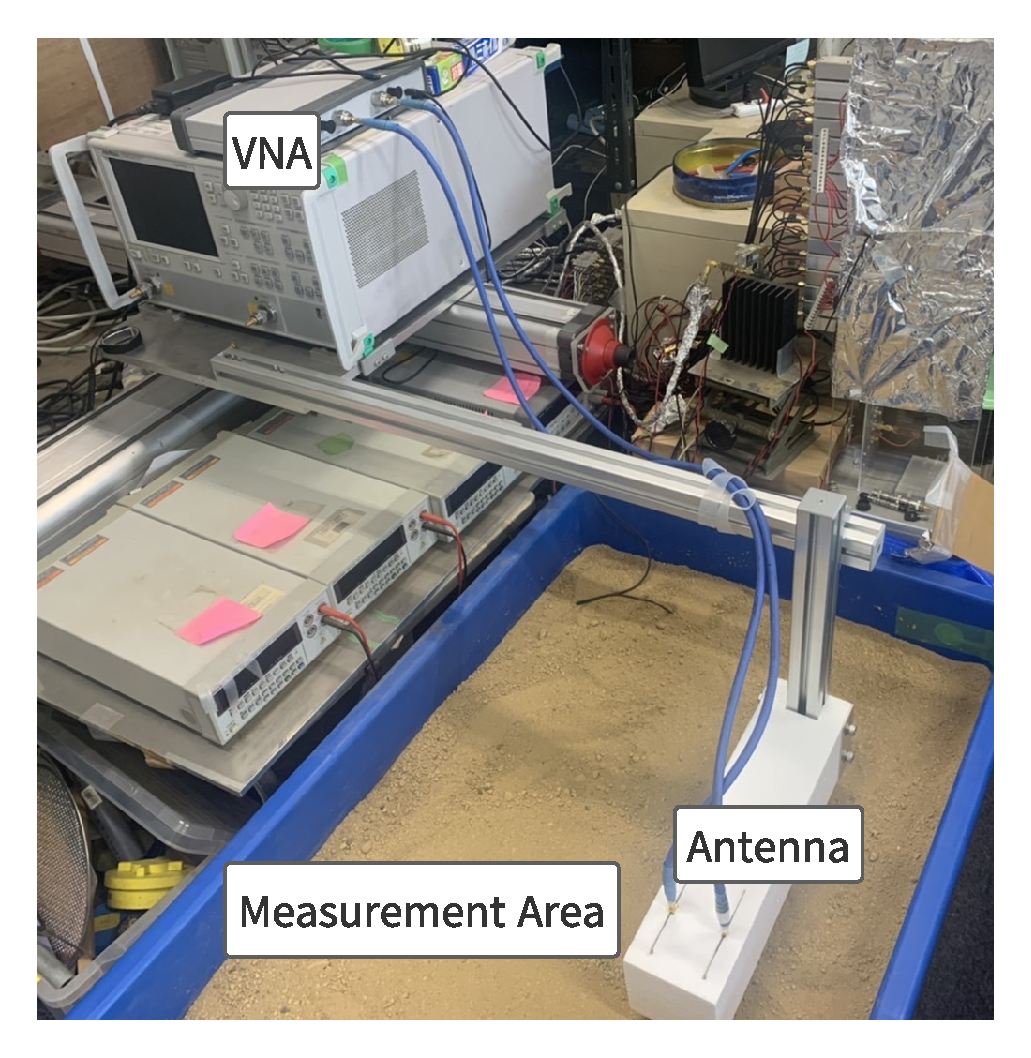
\includegraphics[width=7cm]{./image/Exp_Situ.pdf}
  \caption{実験の様子}\label{実験の様子}
  \end{center}
  \end{figure}

  \begin{figure}[h]
    \begin{center}
     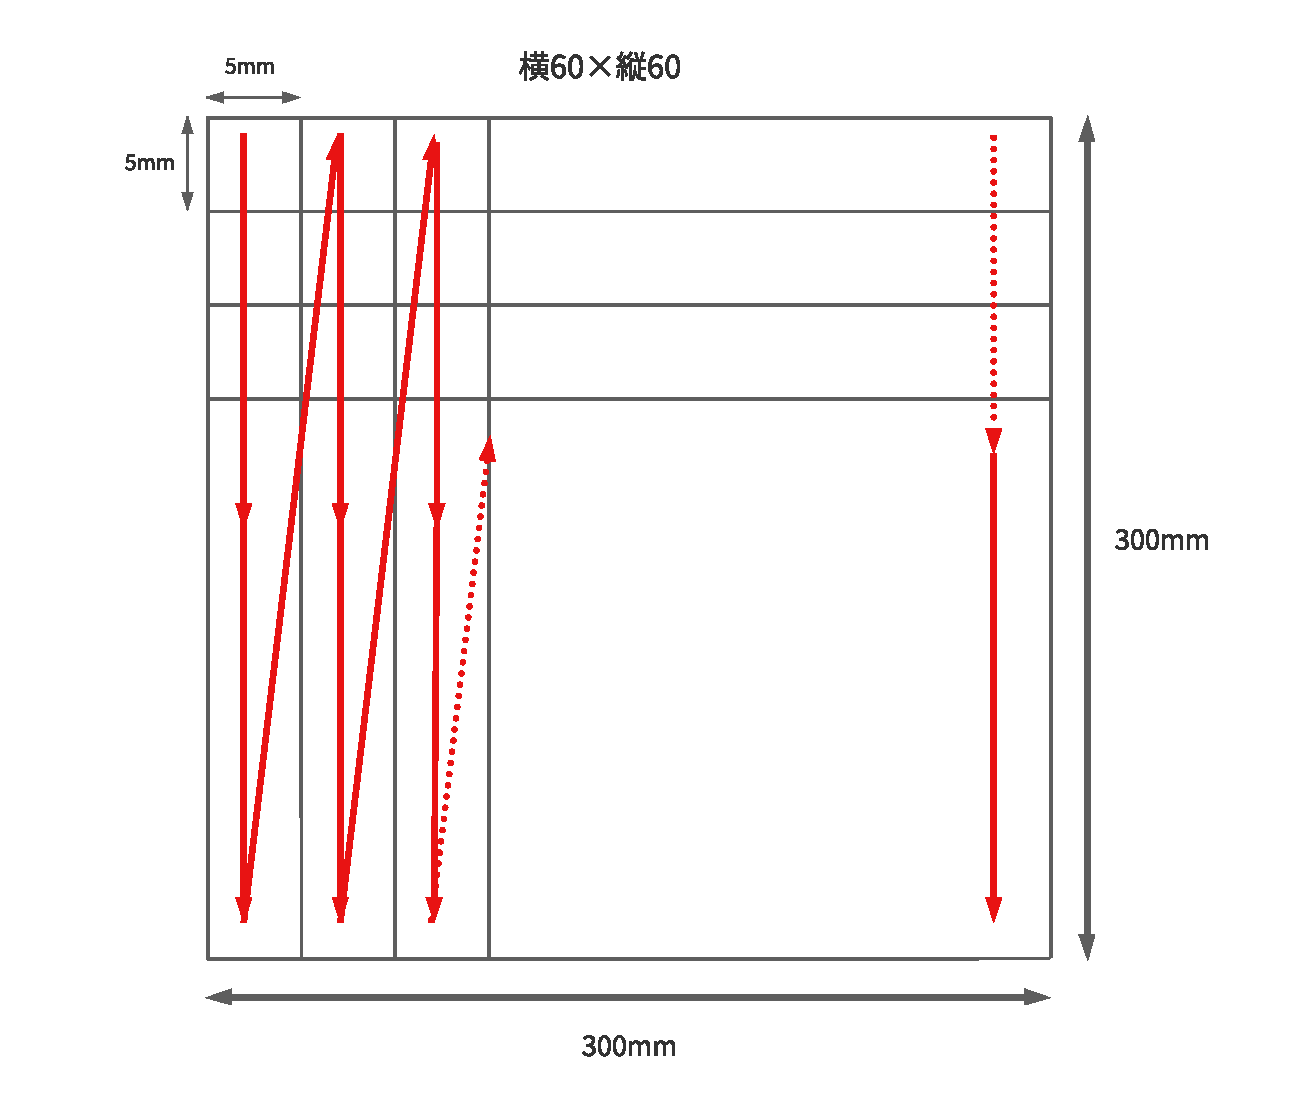
\includegraphics[width=10cm]{./image/sweep.pdf}
    \caption{アンテナの動作方向}\label{アンテナの動作方向}
    \end{center}
    \end{figure}


  \begin{figure}[h]
    \begin{center}
     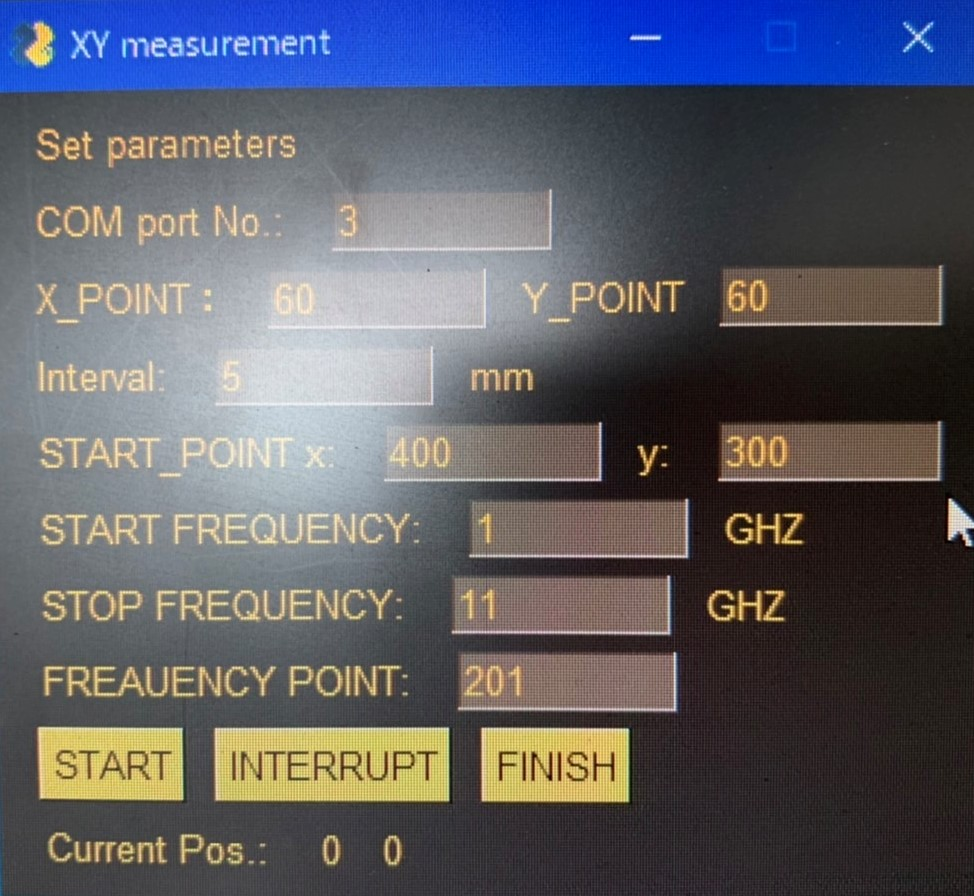
\includegraphics[width=7cm]{./dataimage/exp_image/gui.jpg}
    \caption{データ計測点}\label{データ計測点}
    \end{center}
    \end{figure}

  % \begin{figure}[htbp]
  %   \begin{minipage}[b]{0.45\linewidth}
  %     \centering
  %     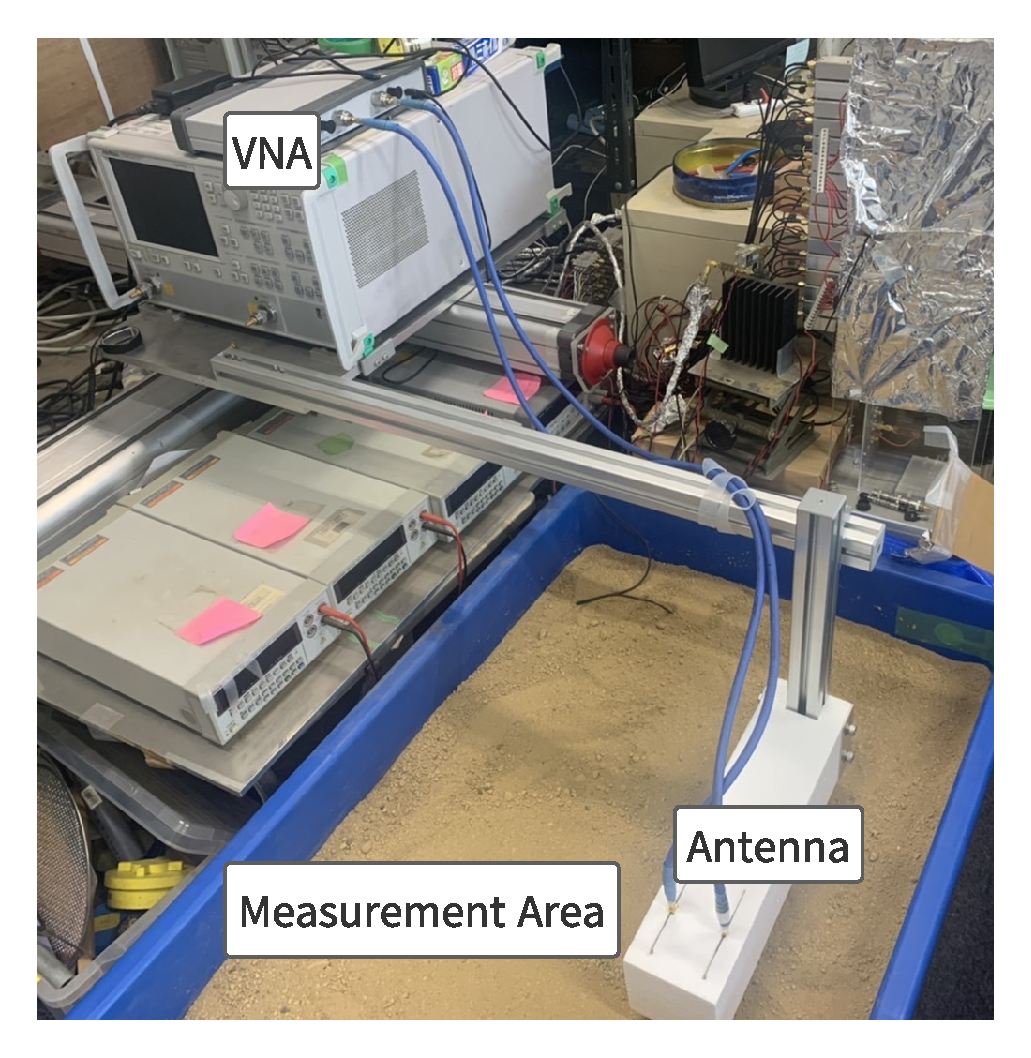
\includegraphics[height=7cm,width=7cm]{./image/Exp_Situ.pdf}
  %     \caption{Composite}
  %   \end{minipage}
  %   \begin{minipage}[b]{0.45\linewidth}
  %     \centering
  %     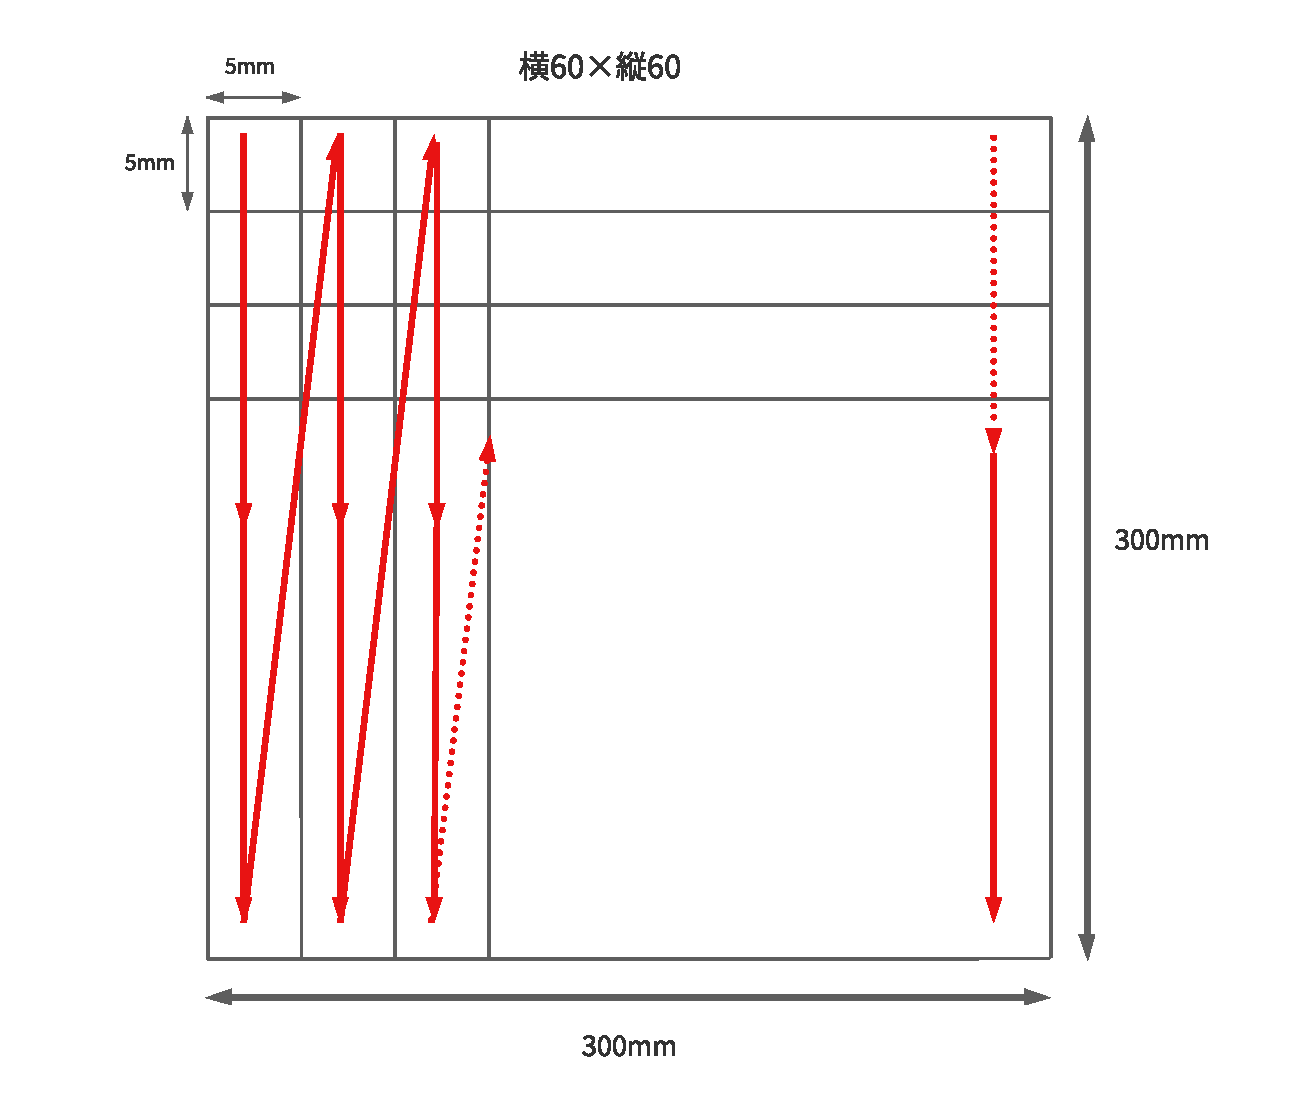
\includegraphics[height=10cm,width=10cm]{./image/sweep.pdf}
  %     \caption{Gradation}
  %   \end{minipage}
  % \end{figure}

  \begin{figure}[htbp]
    \begin{minipage}[b]{0.5\linewidth}
      \centering
      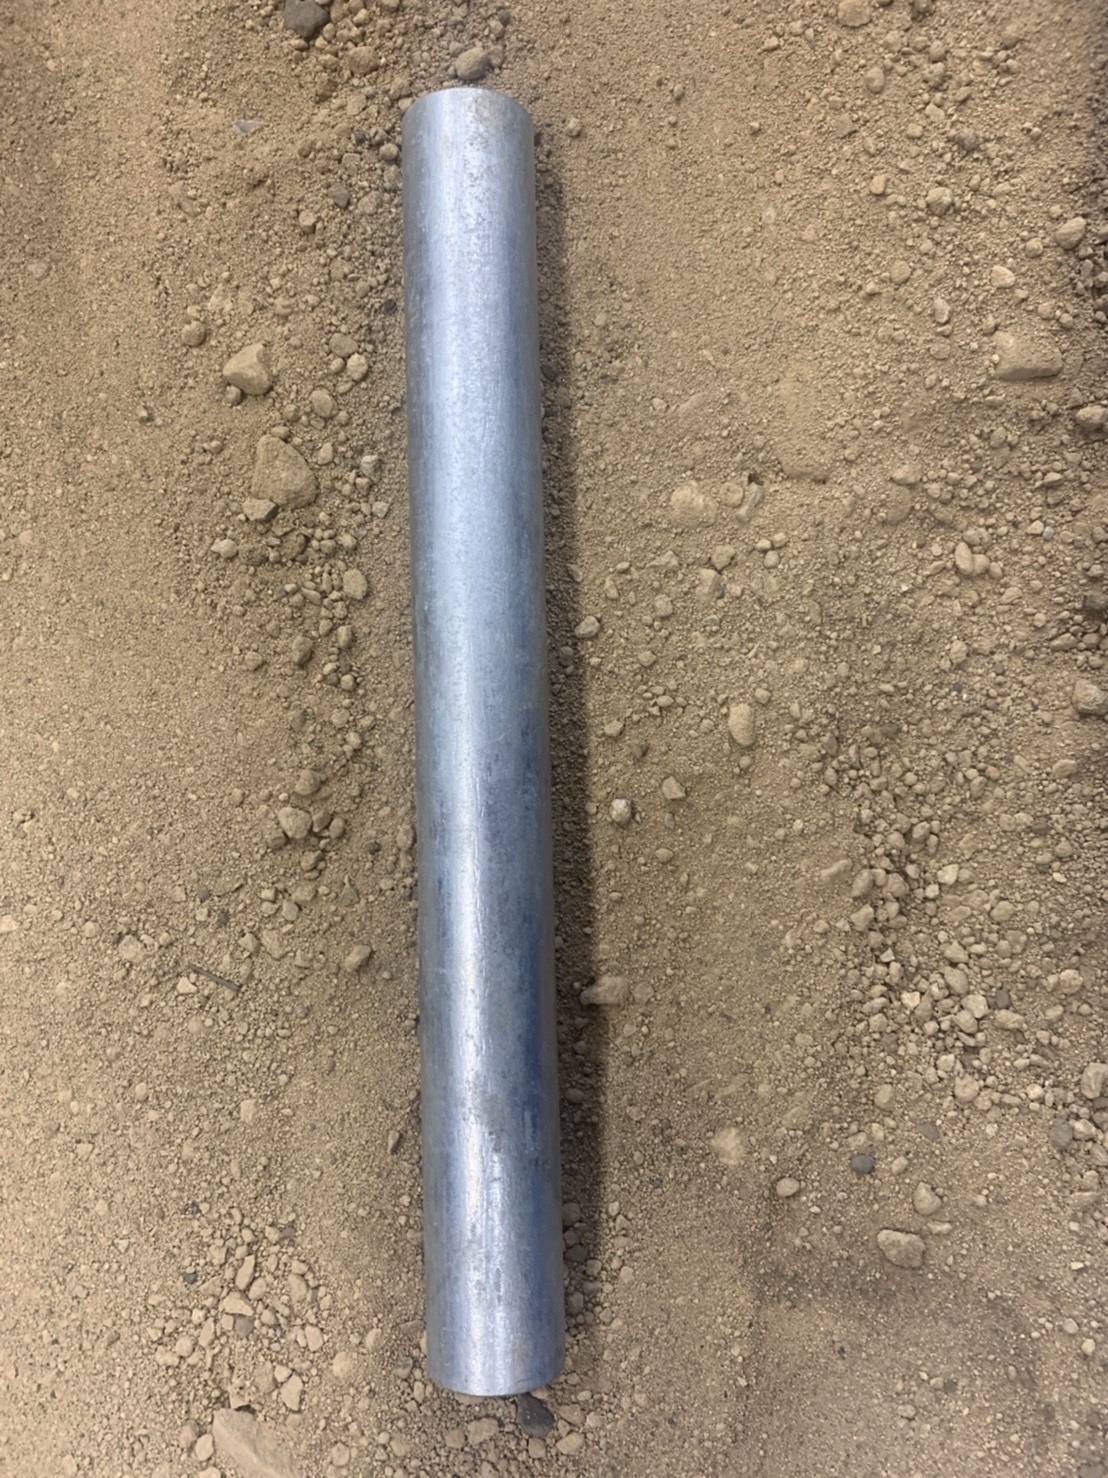
\includegraphics[height=5cm,width=4cm]{dataimage/exp_image/metalpipe.jpg}
      \subcaption{鉄パイプ}
    \end{minipage}
    \begin{minipage}[b]{0.3\linewidth}
      \centering
      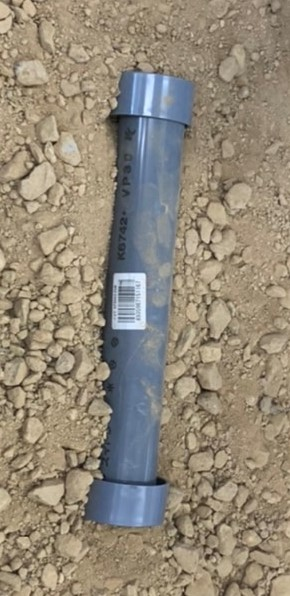
\includegraphics[height=5cm,width=4cm]{dataimage/exp_image/plasticpipe.jpg}
      \subcaption{塩ビ管}
    \end{minipage}
    \caption{埋設したパイプ}
    \label{埋設したパイプ}
  \end{figure}  

  \begin{figure}[h]
    \begin{center}
     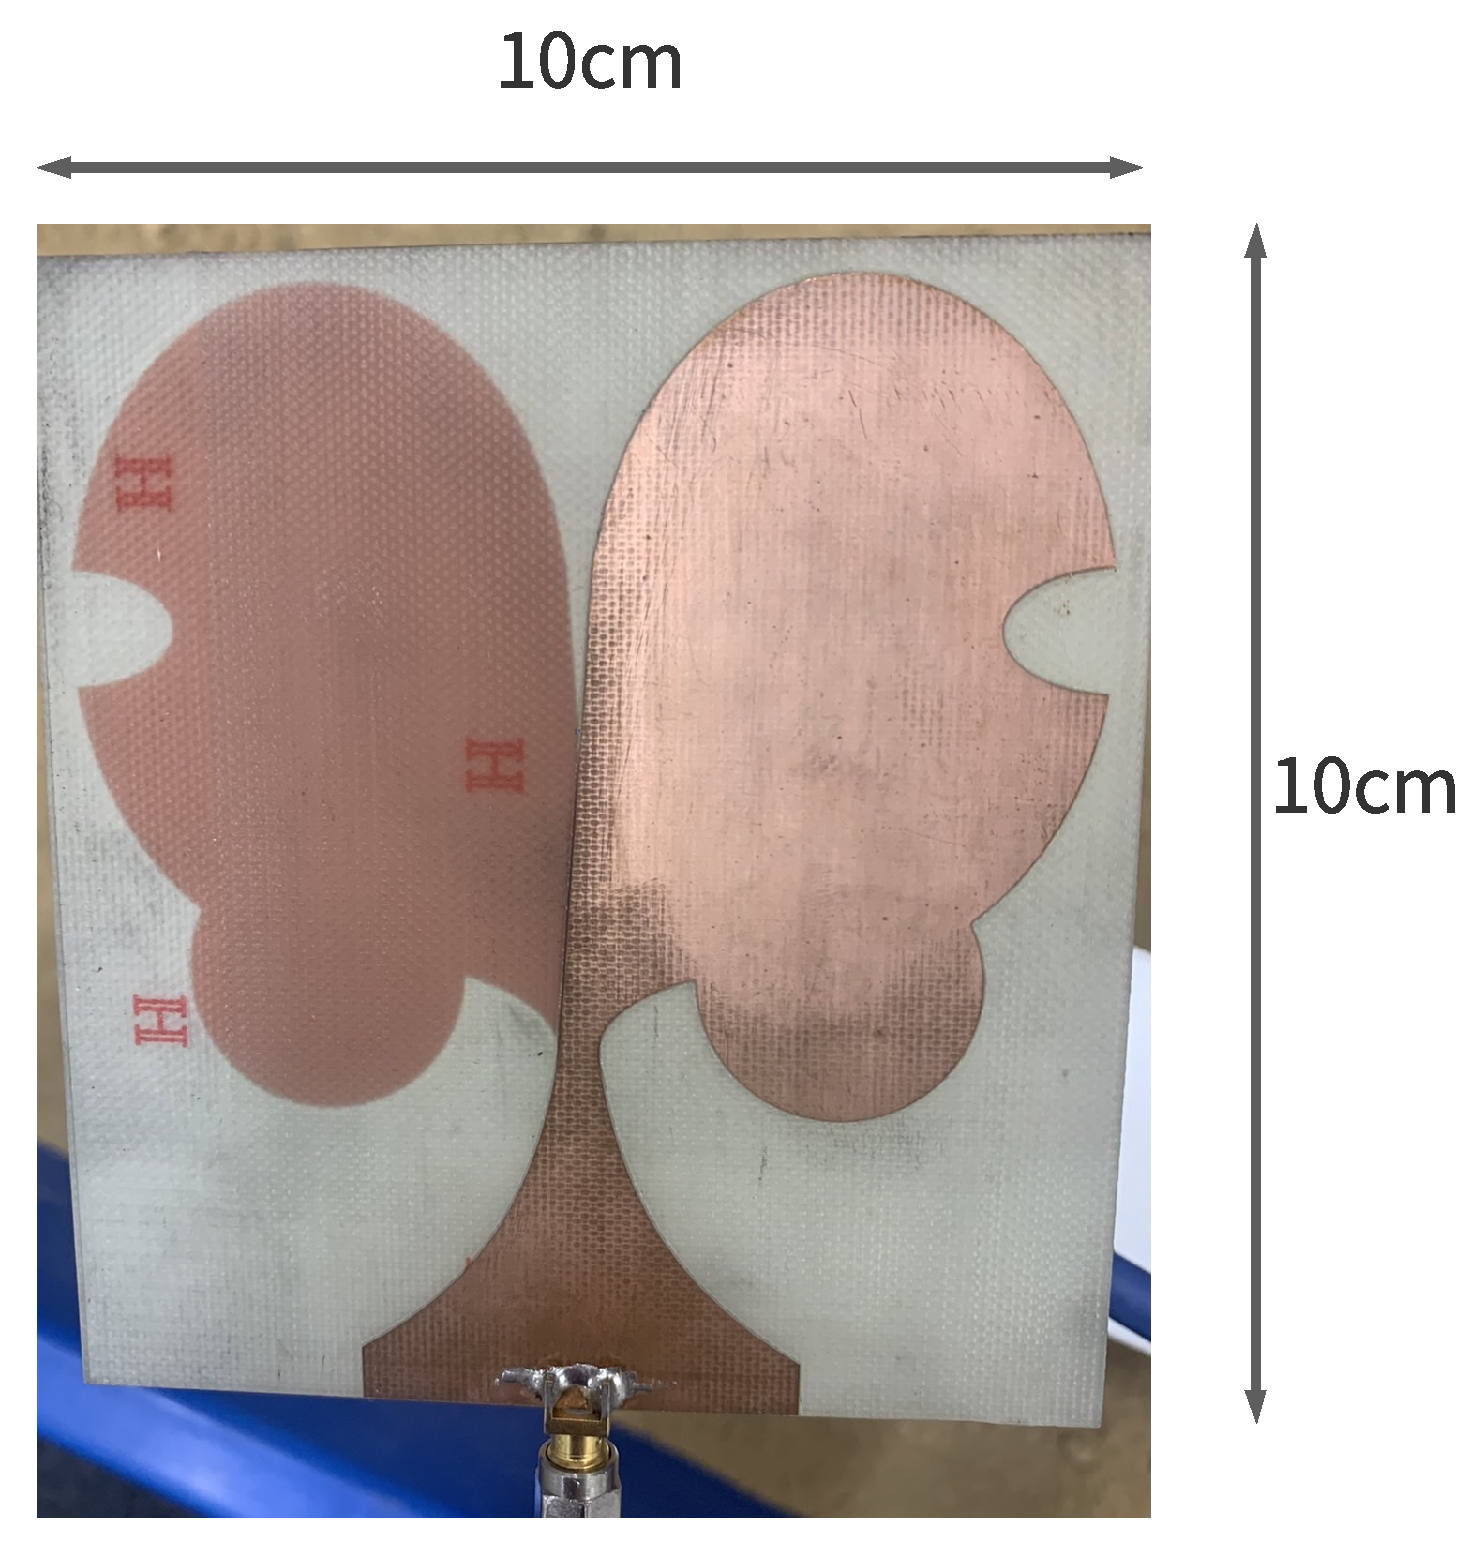
\includegraphics[width=7cm]{./image/antenna.pdf}
    \caption{測定用のアンテナ  }\label{測定用のアンテナ}
    \end{center}
    \end{figure}

\begin{itemize}
\item 普通の$\alpha$は\verb|\alpha|で書く。
\item \verb|$\vec{\alpha}$| で $\vec{\alpha}$
\item \verb|\usepackage{bm}| している場合は
\verb|$\bm{\alpha}$| で $\bm{\alpha}$
\item 並べると,$\alpha$, $\vec{\alpha}$, $\bm{\alpha}$
\end{itemize}

\begin{thebibliography}{99}
 \bibitem{radar1}M.Sato and M.Takeshita,”Estimation of subsurface fracture roughness by
 polarimetric borehole radar,” IEICE Trans. Electron., E83-C,12(2000) 1881-1888
 \bibitem{radar2}T.Moriyama, M.Nakamura, Y.Yamaguchi and H.Yamada,”Radar polarimety applied
 to the classification of target buried in the underground: Wideband Interferometric
 Sensing and Imaging Polarimetry,” Vol.3210 of Proc. of SPIE(1997) 182-189
  \bibitem{phasor}K.Oyama and A.Hirose, "Phasor Quaternion Neural Networks for Singular
  Point Compensation in Polarimetric-Interferometric
  Synthetic Aperture Radar," IEEE Transactions on Geoscience and Remote Sensing, vol. 57, no. 5, May 2019.
  \bibitem{human detection}Y.Kim,  Senior Member, IEEE, and T.Moon, "Human Detection and Activity Classification Based
  on Micro-Doppler Signatures Using Deep
  Convolutional Neural Networks," IEEE Geoscience and Remote Sensing Letters, vol. 13,no. 1,January 2016.
  \bibitem{imai}R.Imai, Y.Song, R.Natsuaki , Senior Member,and A.Hirose, IEEE Transactions on Geoscience and Remote Sensing,
  "Model-Based Homogeneity to Extend Compressed Sensing for Ground Penetrating Radar," vol. 60, 2022.
  \bibitem{hirose1}Y.Nakano and A.Hirose, “Improvement of plastic landmine visualization performance by use of ring-csom and frequency-domain local
  correlation,” IEICE Transactions on Electronics, vol.E92-C, no.1,
  pp.102-108, 2009.
  \bibitem{hirose2}Y.Nakano and A.Hirose, “Adaptive identification of landmine class
  by evaluating the total degree of conformity of ring-SOM,” Australian
  Journal of Intelligent Information Processing Systems, pp.22-28,2010. 
  % http://ajiips.com.au/papers/V12.1/AJIIPS_vol12n1_26-31.pdf
 \bibitem{hirose3}R.Natsuaki and A.Hirose, “Circular property of complex-valued
 correlation learning in CMRF-based filtering for synthetic aperture
 radar interferometry,” Neurocomputing, vol.134, pp.165-172, 2014.
%  https://www.sciencedirect.com/science/article/pii/S092523121400126X

 
  
  % \bibitem{jireishuu}https://geology.co.jp/archives/projects/%E5%9C%B0%E4%B8%AD%E3%83%AC%E3%83%BC%E3%83%80%E3%83%BC%E3%81%AE%E6%96%B0%E3%81%9F%E3%81%AA%E4%BA%8B%E4%BE%8B%E9%9B%86%EF%BC%88%E3%82%B1%E3%83%BC%E3%82%B9%E3%82%B9%E3%82%BF%E3%83%87%E3%82%A3%EF%BC%89#case01

  % \bibitem{satou}http://cobalt.cneas.tohoku.ac.jp/users/sato/newpage24.htm#:~:text=%E5%9C%B0%E4%B8%AD%E3%83%AC%E3%83%BC%E3%83%80%E3%81%AF%E9%9B%BB%E7%A3%81%E6%B3%A2,%E3%83%91%E3%83%BC%E3%82%BD%E3%83%8A%E3%83%AB%E3%83%BB%E3%82%B3%E3%83%B3%E3%83%94%E3%83%A5%E3%83%BC%E3%82%BF%E3%81%A7%E8%A8%98%E9%8C%B2%E3%81%99%E3%82%8B%E3%80%82
  % \bibitem{cs}https://www.innervision.co.jp/ressources/pdf/innervision2014/iv201409_061.pdf
 
  \end{thebibliography}
  
  \end{document}